
%%%%%%%%%%%%%%%%%%%%%%%%%%%%%%%%%%%%%%START PREAMBLE THAT IS THE SAME FOR ALL EXAMPLES
\documentclass{article}

%Required: You must have these
\usepackage{Sweave}
\usepackage{graphicx}
\usepackage{tabularx}
\usepackage{hyperref}

%Optional: I like fancy headers
%\usepackage{fancyhdr}
%\pagestyle{fancy}
%\fancyhead[LO]{Question: How do climate change experiments actually change climate?}
%\fancyhead[RO]{2016}
 %Optional: for outlines
% \usepackage{todonotes}
%%%%%%%%%%%%%%%%%%%%%%%%%%%%%%%%%%%%%%END PREAMBLE THAT IS THE SAME FOR ALL EXAMPLES

%Start of the document
\begin{document}

% \SweaveOpts{concordance=TRUE}

\title{Title: How do climate change experiments actually change climate?} 
\author{A. K. Ettinger,I. Chuine, B. Cook, J. Dukes, A. Ellison, M. Johnston, A. Panetta, C. Rollinson, Y. Vitasse, E. Wolkovich}
%\date{\today}
\maketitle  %put the fancy title on
%%%%%%%%%%%%%%%%%%%%%%%%%%%%%%%%%%%%%%%%%%%%%%%%%%%
\section {Summary}
A Concept/Synthesis Paper with the main message being that climate change experiments need to report what climate variables are modified by their experiment and how, in order to maximize the benefits of these experiments, as well as our understanding of biological impacts of climate change.
\section {Introduction}
Experimental in situ climate manipulations offer several advantages to understanding biological impacts of climate change: (controlled, relative speed- i.e. multiple manipulations can be conducted simultaneously, can hit higher temps, can do them in places where other data collection is hard). 

These advantages come at a cost, however. Experimental in situ climate manipulations are logistically challenging, and expensive. 

Problem:
People want to extrapolate warming experiments to real life to understand (and forecast) biological impacts of climate change. However, a detailed assessment of exactly how experimental warming treatments alter climate, and the extent to which these manipulations accurately model the real world, is lacking. 

\section {Experimental climate change vs. real climate: how do they compare?}
Experimental warming alters climate in several ways that are rarely quantified, summarized, or interpreted in studies reporting on experimental warming, despite the fact that these alterations are likely to have important biological implications.
\subsection  {Structures}
The experimental structures themselves alter temperature, in ways that are not generally examined or reported in experimental warming studies. Compare sham and ambient data on temperature (mixed effects models).
\begin{itemize}
\item Soil temperature is LOWER in the shams, compared with the ambient air. 
%%%%%%%Add figures of sham vs ambient here
\item Air temperature is HIGHER in the shams, compared with the ambient air. 
Below, mean daily soil temperature (for the shallowest depth) and air temperature are shown, for all sites for which these data are available (5-6 sites). 

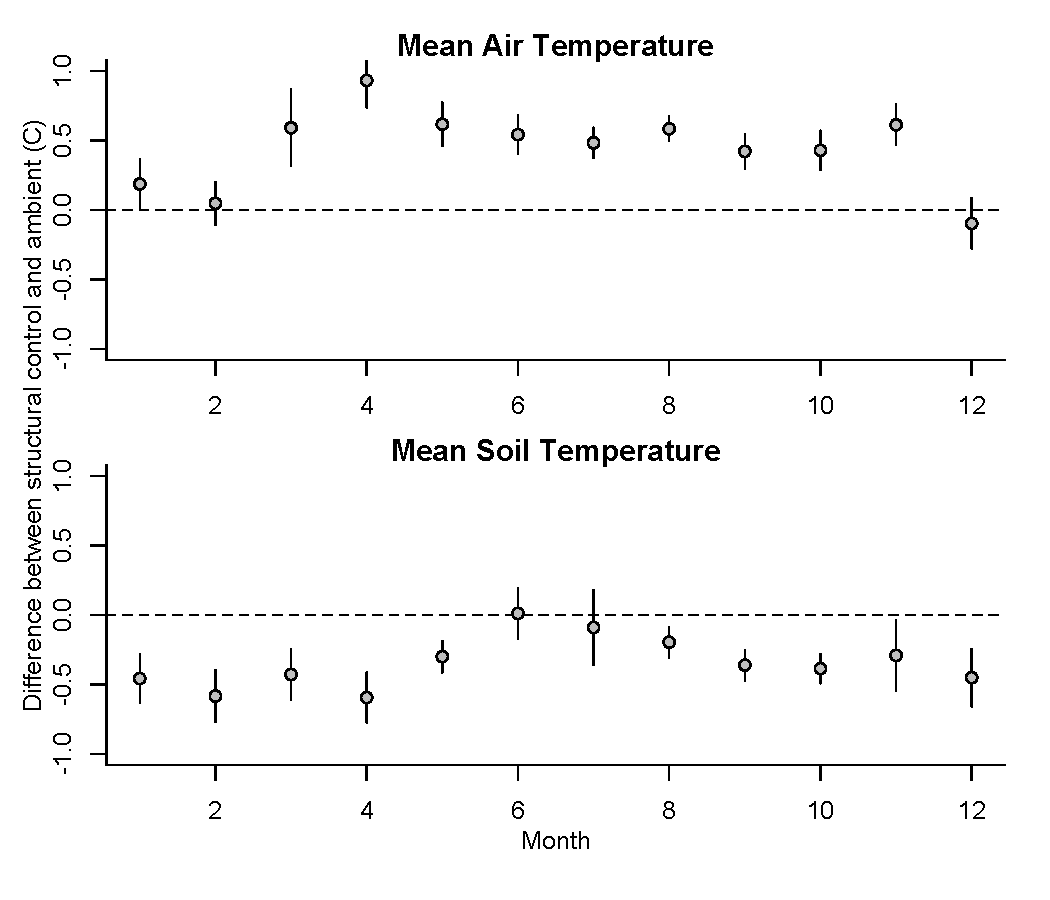
\includegraphics{Analyses/figures/ShamVSAmbient_mean.pdf}
%%%%%%%Add figures of sham vs ambient here
\item The pattern was consistent for min and max air and soil temperatures, as well. See below: 
\end{itemize}
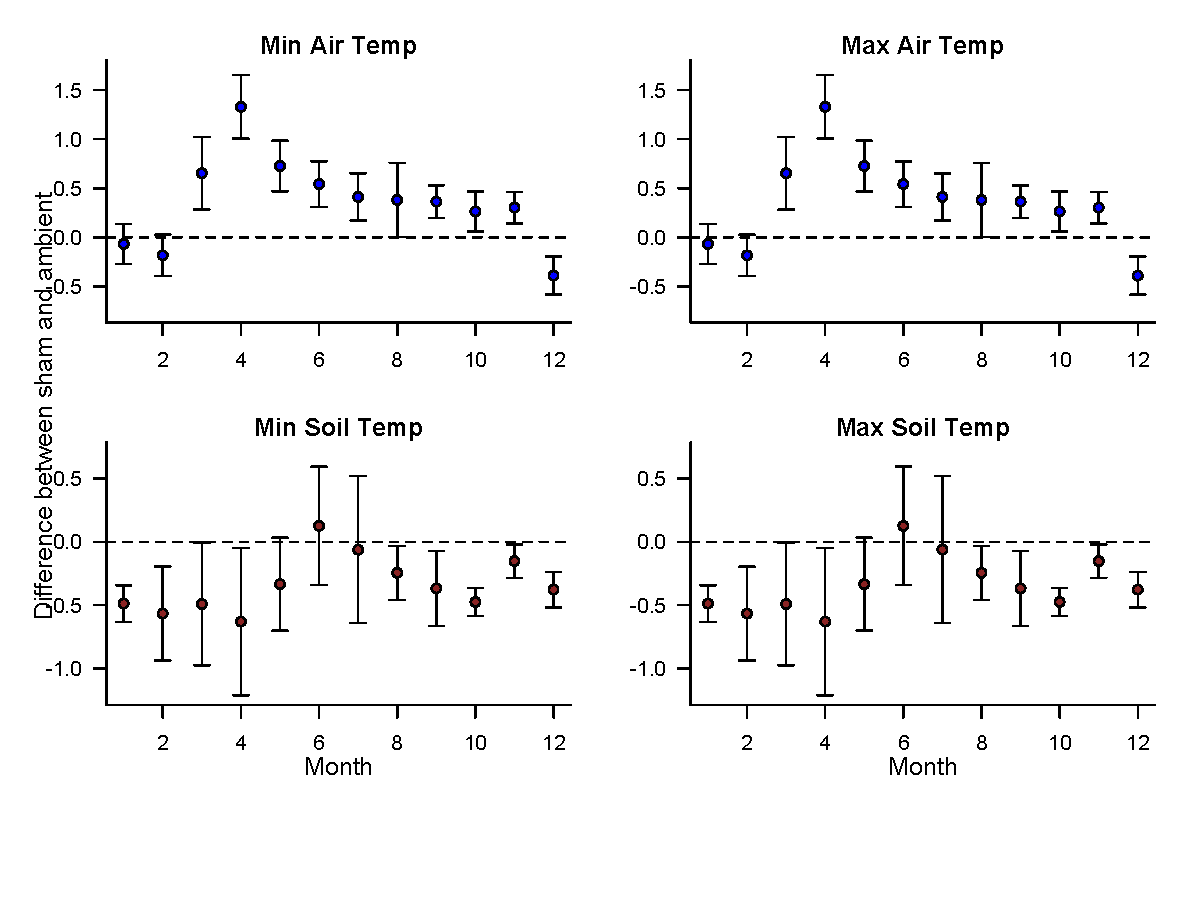
\includegraphics{Analyses/figures/ShamVSAmbient_minmax.pdf}
\subsection{Space}
There is spatial variation in warming effects. Analysis of plot vs. block level variation vs. treatment. also variation within a plot?
\subsection{Time}
\begin{itemize}
\item Seasonal variations in experimental warming effects (plots over time)
\item Daily variations in experimental warming effects (min vs max) 
\item Comparison to observational data: compare warmest years to coolest years. Plot and compare to experimental data
\item Treatments aren?t applied consistently over the year- IR heaters can?t apply consistent warming, and some studies stop warming in different times of year (clark)
\item Secondary effects of warming: Effects of warming on soil moisture (add Miriams analysis here), air humidity, people need to measure these things.
\end{itemize}
\section {Biological Implications}
We have laid out several ways in which experimental warming alters more than just the mean temperature. We argue that these unintended alterations are important for scientists to fully understand and report in their research because they are likely to have biological implications. 
\begin{itemize}
\item For example, plant phenology is likely to be altered in opposing ways by the increased air temperatures and decrease soil moisture/temperature. 
\item Other examples?
\end{itemize}
\section{Recommendations for future climate change experiments}
The criticisms we describe are not meant to imply that experimental warming studies are not worthwhile. On the contrary, we believe that climate change experiments provide invaluable opportunities to isolate how abiotic factors may alter species' performances and interactions. Here we describe a few recommendations to improve future climate change experiments. 
a.	Include controls and collect/use/report their data. Measure before and after experiment, have shams and ambient controls, and collect all data in them
2)	Things everyone should report about their experiments
a.	Control/Sham data
b.	Timing of warming treatment applied (e.g., summer application impacts fall events more): exact date it started and how it ran throughout seasons/years
c.	Day/night variation (across seasons)
d.	Try to collect climate data at least 2X day, ideally hourly
e.	Number of missing data points for warming and why (rodents ate sensors? Heaters went out?)
3)	Regression designs for nonlinearity?
4)	Community standards for reporting experimental climate data (and phenology -Chuine et al. 2017)
5)	Monitoring of temperature that is more useful across designs and that is closest to what focal organisms experience



\end{document}
